First and the most simple analysis was to compare sentiment of tweets collected with period one week. I have also added the sentiment of some projects' Reddit discussions (keep in mind that classifier is trained on tweets, so this is not the best approach). Results can be seen in Table \ref{table:weeklyAverageTable} and Figure \ref{fig:weeklyAverageBarchart}

\begin{table}[H]
\centering
\begin{tabular}{ |p{2cm}|p{5.5cm}|p{5.5cm}|}
 \hline
\textbf{Project }& \textbf{Twitter average sentiment} & \textbf{Reddit average sentiment}\\
 \hline
 NodeJS   & 0.697   & 0.633 \\ \hline
 EmberJS   & 0.709   & 0.69\\ \hline
 VueJS   & 0.715   & 0.60\\ \hline 
 Symfony & 0.727   & *\\ \hline   
 AngularJS   & 0.727   & 0.618\\ \hline
 CakePhp & 0.703  & * \\ \hline 
 Bower   & 0.641   & No subreddit\\ \hline 
 Laravel & 0.701   & *\\ \hline
 Gulp & 0.578   & No subreddit\\ \hline
 Yii & 0.658  & * \\ \hline
 Bootstrap & 0.713  & 0.635\\ \hline
 \multicolumn{3}{l}{* Reddit changed its API and submissions endpoint is not supported anymore}
\end{tabular}
\caption{Average sentiment of tweets collected weekly}
\label{table:weeklyAverageTable}
\end{table}


\begin{figure}[H]%
    \centering
	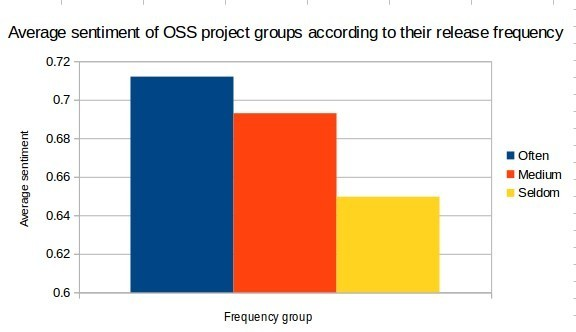
\includegraphics[width=11cm]{weeklyAverageBarchart.jpg}
    \caption{Average sentiment of OSS project groups according to their release frequency}%
    \label{fig:weeklyAverageBarchart}%
\end{figure}

In both of previous analysis, I have used the simplest aggregation operation which is average. Replacing this one with median, modus or some more advanced aggregations could potentially yield different results but because each group is represented just by 3 or 4 OSS projects, losing any data would actually be a significant part of the overall analysed dataset. Using more projects could be potentially a part of future work.